\documentclass{article}
% Some basic packages
\usepackage[utf8]{inputenc}
\usepackage[T1]{fontenc}
\usepackage{textcomp}
\usepackage[dutch]{babel}
\usepackage{url}
\usepackage{graphicx}
\usepackage{float}
\usepackage{booktabs}
\usepackage{enumitem}

\pdfminorversion=7

% Don't indent paragraphs, leave some space between them
\usepackage{parskip}

% Hide page number when page is empty
\usepackage{emptypage}
\usepackage{subcaption}
\usepackage{multicol}
\usepackage{xcolor}

% Other font I sometimes use.
% \usepackage{cmbright}

% Math stuff
\usepackage{amsmath, amsfonts, mathtools, amsthm, amssymb}
% Fancy script capitals
\usepackage{mathrsfs}
\usepackage{cancel}
% Bold math
\usepackage{bm}
% Some shortcuts
\newcommand\N{\ensuremath{\mathbb{N}}}
\newcommand\R{\ensuremath{\mathbb{R}}}
\newcommand\Z{\ensuremath{\mathbb{Z}}}
\renewcommand\O{\ensuremath{\emptyset}}
\newcommand\Q{\ensuremath{\mathbb{Q}}}
\newcommand\C{\ensuremath{\mathbb{C}}}

% Easily typeset systems of equations (French package)
\usepackage{systeme}

% Put x \to \infty below \lim
\let\svlim\lim\def\lim{\svlim\limits}

%Make implies and impliedby shorter
\let\implies\Rightarrow
\let\impliedby\Leftarrow
\let\iff\Leftrightarrow
\let\epsilon\varepsilon

% Add \contra symbol to denote contradiction
\usepackage{stmaryrd} % for \lightning
\newcommand\contra{\scalebox{1.5}{$\lightning$}}

% \let\phi\varphi

% Command for short corrections
% Usage: 1+1=\correct{3}{2}

\definecolor{correct}{HTML}{009900}
\newcommand\correct[2]{\ensuremath{\:}{\color{red}{#1}}\ensuremath{\to }{\color{correct}{#2}}\ensuremath{\:}}
\newcommand\green[1]{{\color{correct}{#1}}}

% horizontal rule
\newcommand\hr{
    \noindent\rule[0.5ex]{\linewidth}{0.5pt}
}

% hide parts
\newcommand\hide[1]{}

% si unitx
\usepackage{siunitx}
\sisetup{locale = FR}

% Environments
\makeatother
% For box around Definition, Theorem, \ldots
\usepackage{mdframed}
\mdfsetup{skipabove=1em,skipbelow=0em}
\theoremstyle{definition}
\newmdtheoremenv[nobreak=true]{definitie}{Definitie}
\newmdtheoremenv[nobreak=true]{eigenschap}{Eigenschap}
\newmdtheoremenv[nobreak=true]{gevolg}{Gevolg}
\newmdtheoremenv[nobreak=true]{lemma}{Lemma}
\newmdtheoremenv[nobreak=true]{propositie}{Propositie}
\newmdtheoremenv[nobreak=true]{stelling}{Stelling}
\newmdtheoremenv[nobreak=true]{wet}{Wet}
\newmdtheoremenv[nobreak=true]{postulaat}{Postulaat}
\newmdtheoremenv{conclusie}{Conclusie}
\newmdtheoremenv{toemaatje}{Toemaatje}
\newmdtheoremenv{vermoeden}{Vermoeden}
\newtheorem*{herhaling}{Herhaling}
\newtheorem*{intermezzo}{Intermezzo}
\newtheorem*{notatie}{Notatie}
\newtheorem*{observatie}{Observatie}
\newtheorem*{oef}{Oefening}
\newtheorem*{opmerking}{Opmerking}
\newtheorem*{praktisch}{Praktisch}
\newtheorem*{probleem}{Probleem}
\newtheorem*{terminologie}{Terminologie}
\newtheorem*{toepassing}{Toepassing}
\newtheorem*{uovt}{UOVT}
\newtheorem*{vb}{Voorbeeld}
\newtheorem*{vraag}{Vraag}

\newmdtheoremenv[nobreak=true]{definition}{Definition}
\newtheorem*{eg}{Example}
\newtheorem*{notation}{Notation}
\newtheorem*{previouslyseen}{As previously seen}
\newtheorem*{remark}{Remark}
\newtheorem*{note}{Note}
\newtheorem*{problem}{Problem}
\newtheorem*{observe}{Observe}
\newtheorem*{property}{Property}
\newtheorem*{intuition}{Intuition}
\newmdtheoremenv[nobreak=true]{prop}{Proposition}
\newmdtheoremenv[nobreak=true]{theorem}{Theorem}
\newmdtheoremenv[nobreak=true]{corollary}{Corollary}

% End example and intermezzo environments with a small diamond (just like proof
% environments end with a small square)
\usepackage{etoolbox}
\AtEndEnvironment{vb}{\null\hfill$\diamond$}%
\AtEndEnvironment{intermezzo}{\null\hfill$\diamond$}%
% \AtEndEnvironment{opmerking}{\null\hfill$\diamond$}%

% Fix some spacing
% http://tex.stackexchange.com/questions/22119/how-can-i-change-the-spacing-before-theorems-with-amsthm
\makeatletter
\def\thm@space@setup{%
  \thm@preskip=\parskip \thm@postskip=0pt
}


% Exercise 
% Usage:
% \oefening{5}
% \suboefening{1}
% \suboefening{2}
% \suboefening{3}
% gives
% Oefening 5
%   Oefening 5.1
%   Oefening 5.2
%   Oefening 5.3
\newcommand{\oefening}[1]{%
    \def\@oefening{#1}%
    \subsection*{Oefening #1}
}

\newcommand{\suboefening}[1]{%
    \subsubsection*{Oefening \@oefening.#1}
}


% \lecture starts a new lecture (les in dutch)
%
% Usage:
% \lecture{1}{di 12 feb 2019 16:00}{Inleiding}
%
% This adds a section heading with the number / title of the lecture and a
% margin paragraph with the date.

% I use \dateparts here to hide the year (2019). This way, I can easily parse
% the date of each lecture unambiguously while still having a human-friendly
% short format printed to the pdf.

\usepackage{xifthen}
\def\testdateparts#1{\dateparts#1\relax}
\def\dateparts#1 #2 #3 #4 #5\relax{
    \marginpar{\small\textsf{\mbox{#1 #2 #3 #5}}}
}

\def\@lecture{}%
\newcommand{\lecture}[3]{
    \ifthenelse{\isempty{#3}}{%
        \def\@lecture{Lecture #1}%
    }{%
        \def\@lecture{Lecture #1: #3}%
    }%
    \subsection*{\@lecture}
    \marginpar{\small\textsf{\mbox{#2}}}
}



% These are the fancy headers
\usepackage{fancyhdr}
\pagestyle{fancy}

% LE: left even
% RO: right odd
% CE, CO: center even, center odd
% My name for when I print my lecture notes to use for an open book exam.
% \fancyhead[LE,RO]{Isidoor Pinillo Esquivel}

\fancyhead[RO,LE]{\@lecture} % Right odd,  Left even
\fancyhead[RE,LO]{}          % Right even, Left odd

\fancyfoot[RO,LE]{\thepage}  % Right odd,  Left even
\fancyfoot[RE,LO]{}          % Right even, Left odd
\fancyfoot[C]{\leftmark}     % Center

\makeatother




% Todonotes and inline notes in fancy boxes
\usepackage{todonotes}
\usepackage{tcolorbox}

% Make boxes breakable
\tcbuselibrary{breakable}

% Verbetering is correction in Dutch
% Usage: 
% \begin{verbetering}
%     Lorem ipsum dolor sit amet, consetetur sadipscing elitr, sed diam nonumy eirmod
%     tempor invidunt ut labore et dolore magna aliquyam erat, sed diam voluptua. At
%     vero eos et accusam et justo duo dolores et ea rebum. Stet clita kasd gubergren,
%     no sea takimata sanctus est Lorem ipsum dolor sit amet.
% \end{verbetering}
\newenvironment{verbetering}{\begin{tcolorbox}[
    arc=0mm,
    colback=white,
    colframe=green!60!black,
    title=Opmerking,
    fonttitle=\sffamily,
    breakable
]}{\end{tcolorbox}}

% Noot is note in Dutch. Same as 'verbetering' but color of box is different
\newenvironment{noot}[1]{\begin{tcolorbox}[
    arc=0mm,
    colback=white,
    colframe=white!60!black,
    title=#1,
    fonttitle=\sffamily,
    breakable
]}{\end{tcolorbox}}




% Figure support as explained in my blog post.
\usepackage{import}
\usepackage{xifthen}
\usepackage{pdfpages}
\usepackage{transparent}
\newcommand{\incfig}[1]{%
    \def\svgwidth{\columnwidth}
    \import{./figures/}{#1.pdf_tex}
}

% Fix some stuff
% %http://tex.stackexchange.com/questions/76273/multiple-pdfs-with-page-group-included-in-a-single-page-warning
\pdfsuppresswarningpagegroup=1


% My name
\author{Isidoor Pinillo Esquivel}

\usepackage{graphicx}

\begin{document}
\oefening{1}

We gaan de Black-Scholes PDE in het
discretisatie rooster $(s_{i})$ beschouwen
met volgende notatie.
  \begin{align*}
    u',u'_{j}   &= u_{t},u_{t}(s_{j},t)\\
    c^{2},c^{1},c^{0}&= \frac{1}{2} \sigma^{2}s^{2}, rs , r  
  \end{align*}
 Benaderingen van $u$ zullen aangeduid worden met
 $U$.

De Black-Scholes vergelijking met deze notatie wordt:
\[
  u'= c_{2}u_{ss }+ c_{1}u_{s} -c_{0}u
.\]

Dit zijn tweede orde benaderingen voor de afgeleiden van $u$ (tweede orde centraal):

\begin{align*}
  u_{s}  &= \frac{u(s+h)-u(s-h)}{2h} + O(h^{2})\\
  u_{ss} &= \frac{u(s+h)-2u(s)+u(s-h)}{h^{2}} + O(h^{2})
\end{align*}

Hiermee wordt de benaderde Black-Scholes vergelijking
in het rooster:

\[
  U'_{j}= \frac{c_{j}^{2}}{h^{2}}(U_{j+1}-2U_{j}+ U_{j-1})
  + \frac{c_{j}^{1}}{2h}(U_{j+1}-U_{j-1})
  - c_{j}^{0}U_{j} 
.\]
Dit kunnen we eenvoudiger schrijven in matrix vorm.
Voer eerst volgende notatie in 
\[
    D_{j}=
  \left[
  \left(
  \frac{c_{j}^{2}}{h^{2}} + \frac{c_{j}^{1}}{2h}
  \right) ,
  \left(
  -2 \frac{c_{j}^{2}}{h^{2}}- c_{j}^{0}
  \right) ,
  \left(
  \frac{c_{j}^{2}}{h^{2}} - \frac{c_{j}^{1}}{2h} 
  \right) 
  \right]  .\]
Hiermee wordt dit
\[
U'_{j}=D_{j} \left( U_{j-1},U_{j}, U_{j+1} \right)^{T}
 \text{voor } 1 \le j \le m.\]
Nog meer notatie
\begin{align*}
  U' &= (U'_{1}, U'_{2}, ..., U'_{m})^{T}\\
  U_{d} &= (U_{0}, U_{2}, ..., U_{m+1})^{T}\\
  A_{d} &= \text{Diag}(D_{j})\\
  U &= U_{d}\text{ zonder de eerste en laatste rij } \\
  A &= A_{d}\text{ zonder de eerste en laatste kolom} 
\end{align*}
Hiermee wordt dit
\[
  U' = A_{d}U_{d}
.\]

Door de beginvoorwaarden zijn we enkel geïnteresseerd
in $U$. Door de structuur van $A_{d}$ en de 
beginvoorwaarden kunnen we $U_{0}$
en $U_{m+1}$ wegwerken in een term $g(t)$.

\[
  U' = AU + (D_{1})_{0}U_{0}e_{1} + (D_{m})_{2} U_{m+1} e_{m}
.\]

Merk op dat in deze opgave $U_{0}=0$.
\oefening{2}
Kijk naar figuur\ref{fig:mnexp} voor de gevraagde grafiek. Dit suggereert 
dat $\omega = 0$ en $K = 2$ stabiliteit constanten
zijn voor deze semi discretisatie. \\
Als $m \rightarrow \infty$ dan wordt de bijhorende grafiek waarschijnlijk
een rechte.

\begin{figure}
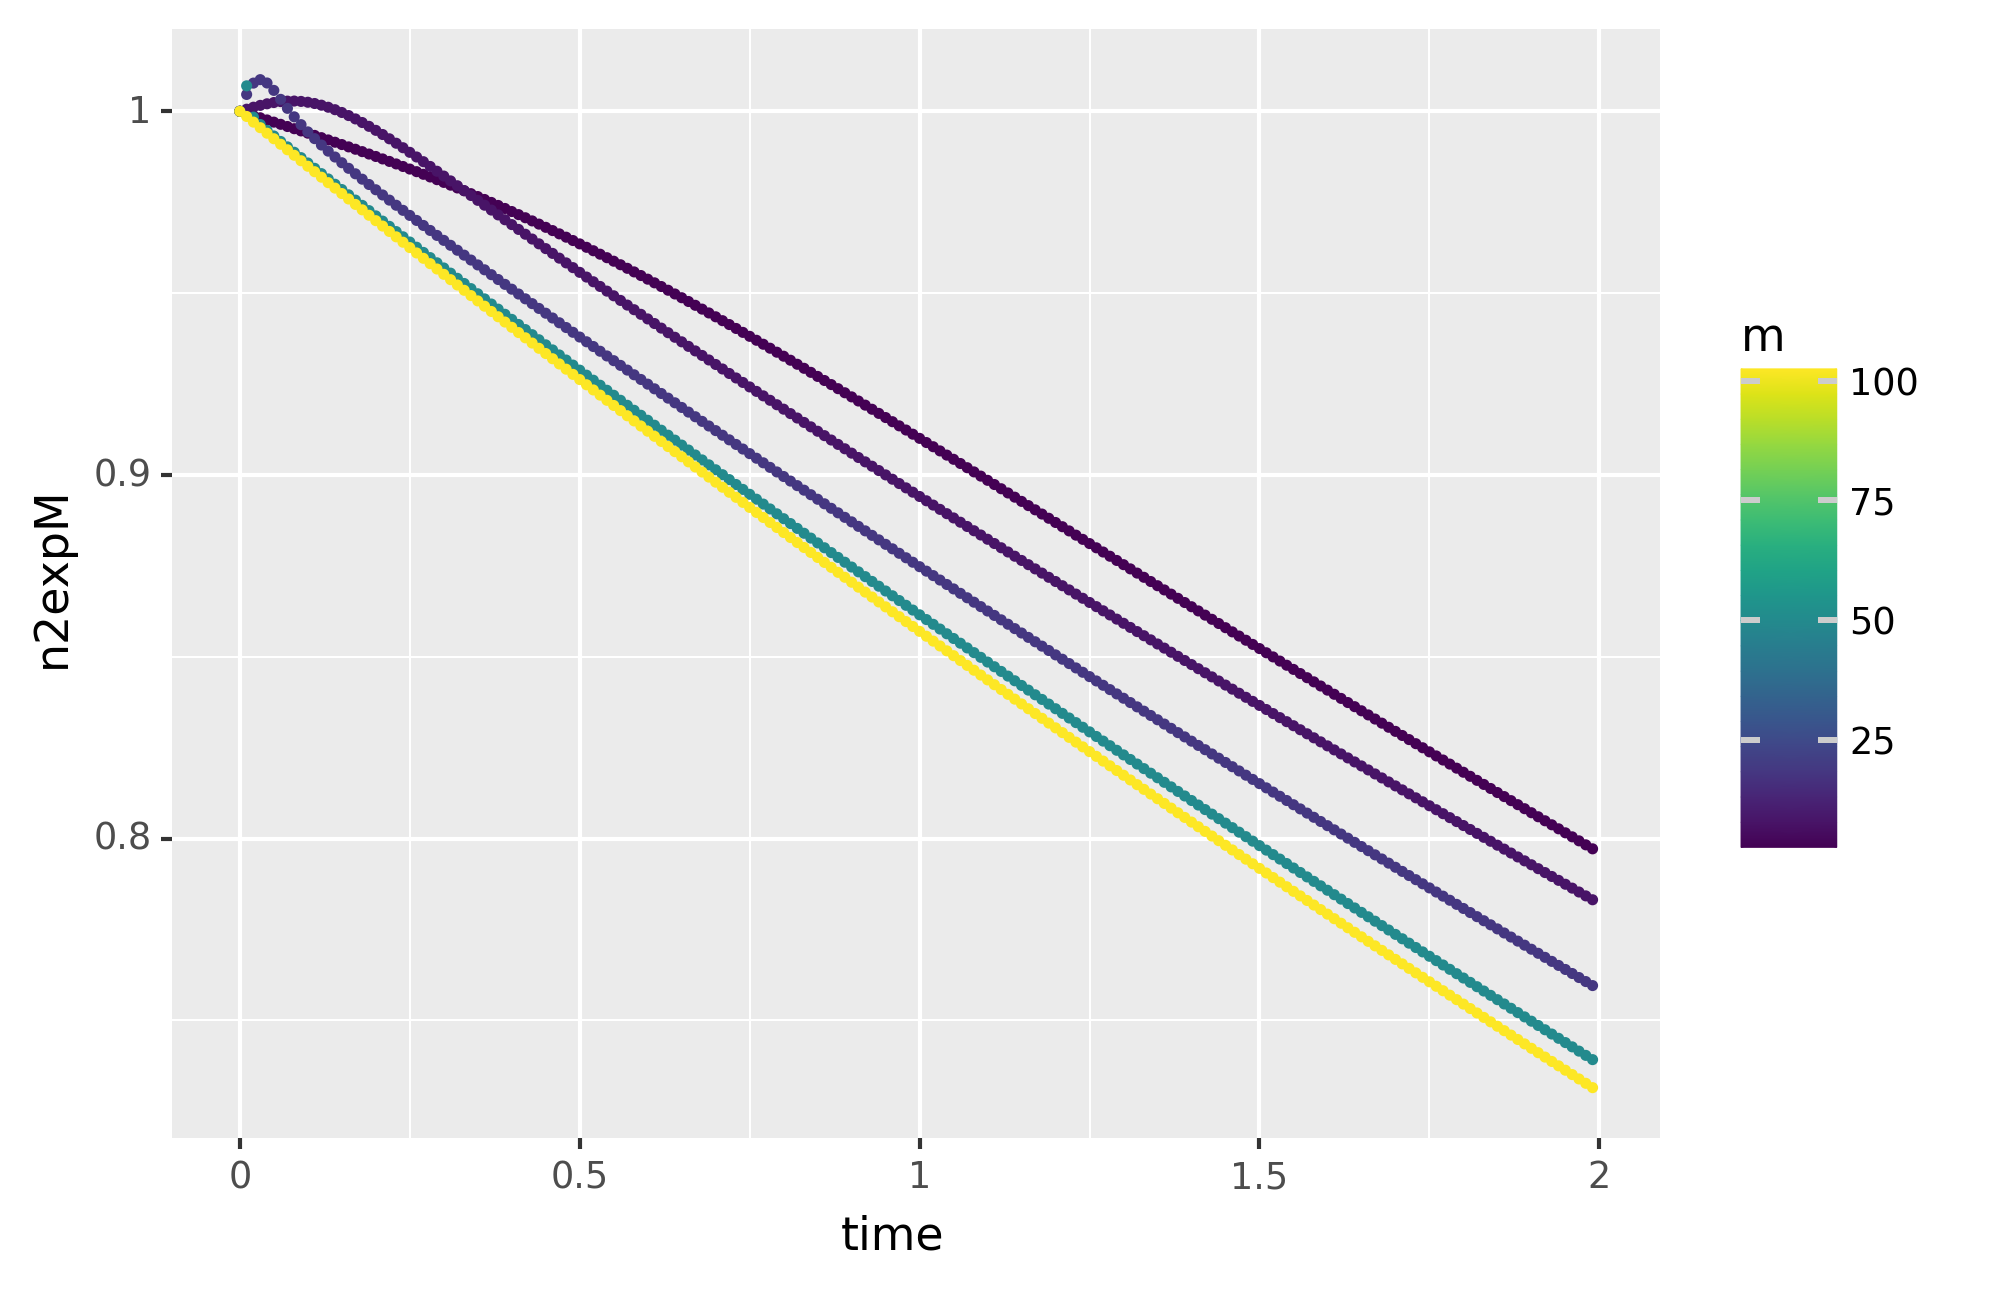
\includegraphics[width=\linewidth]{oefening2.png}
\caption{ $||e^{At}||_{2}$ vs $t$ voor verschillende $m$}\label{fig:mnexp}
\end{figure}

\oefening{3}
Kijk naar figuur\ref{fig:muA} voor $\mu_{2}(A)$ voor verschillende $m$. 
$\mu_{2}(A)$ groeit even snel als $m^{2}$ (kijk grafiek). Dit kan waarschijnlijk
bewezen worden met $\mu_{1}, \mu_{2}$ afschatting. Dit betekent dat voor  
$K$ de stabiliteit constante bij $T = \infty: K > 1$ .

\begin{figure}
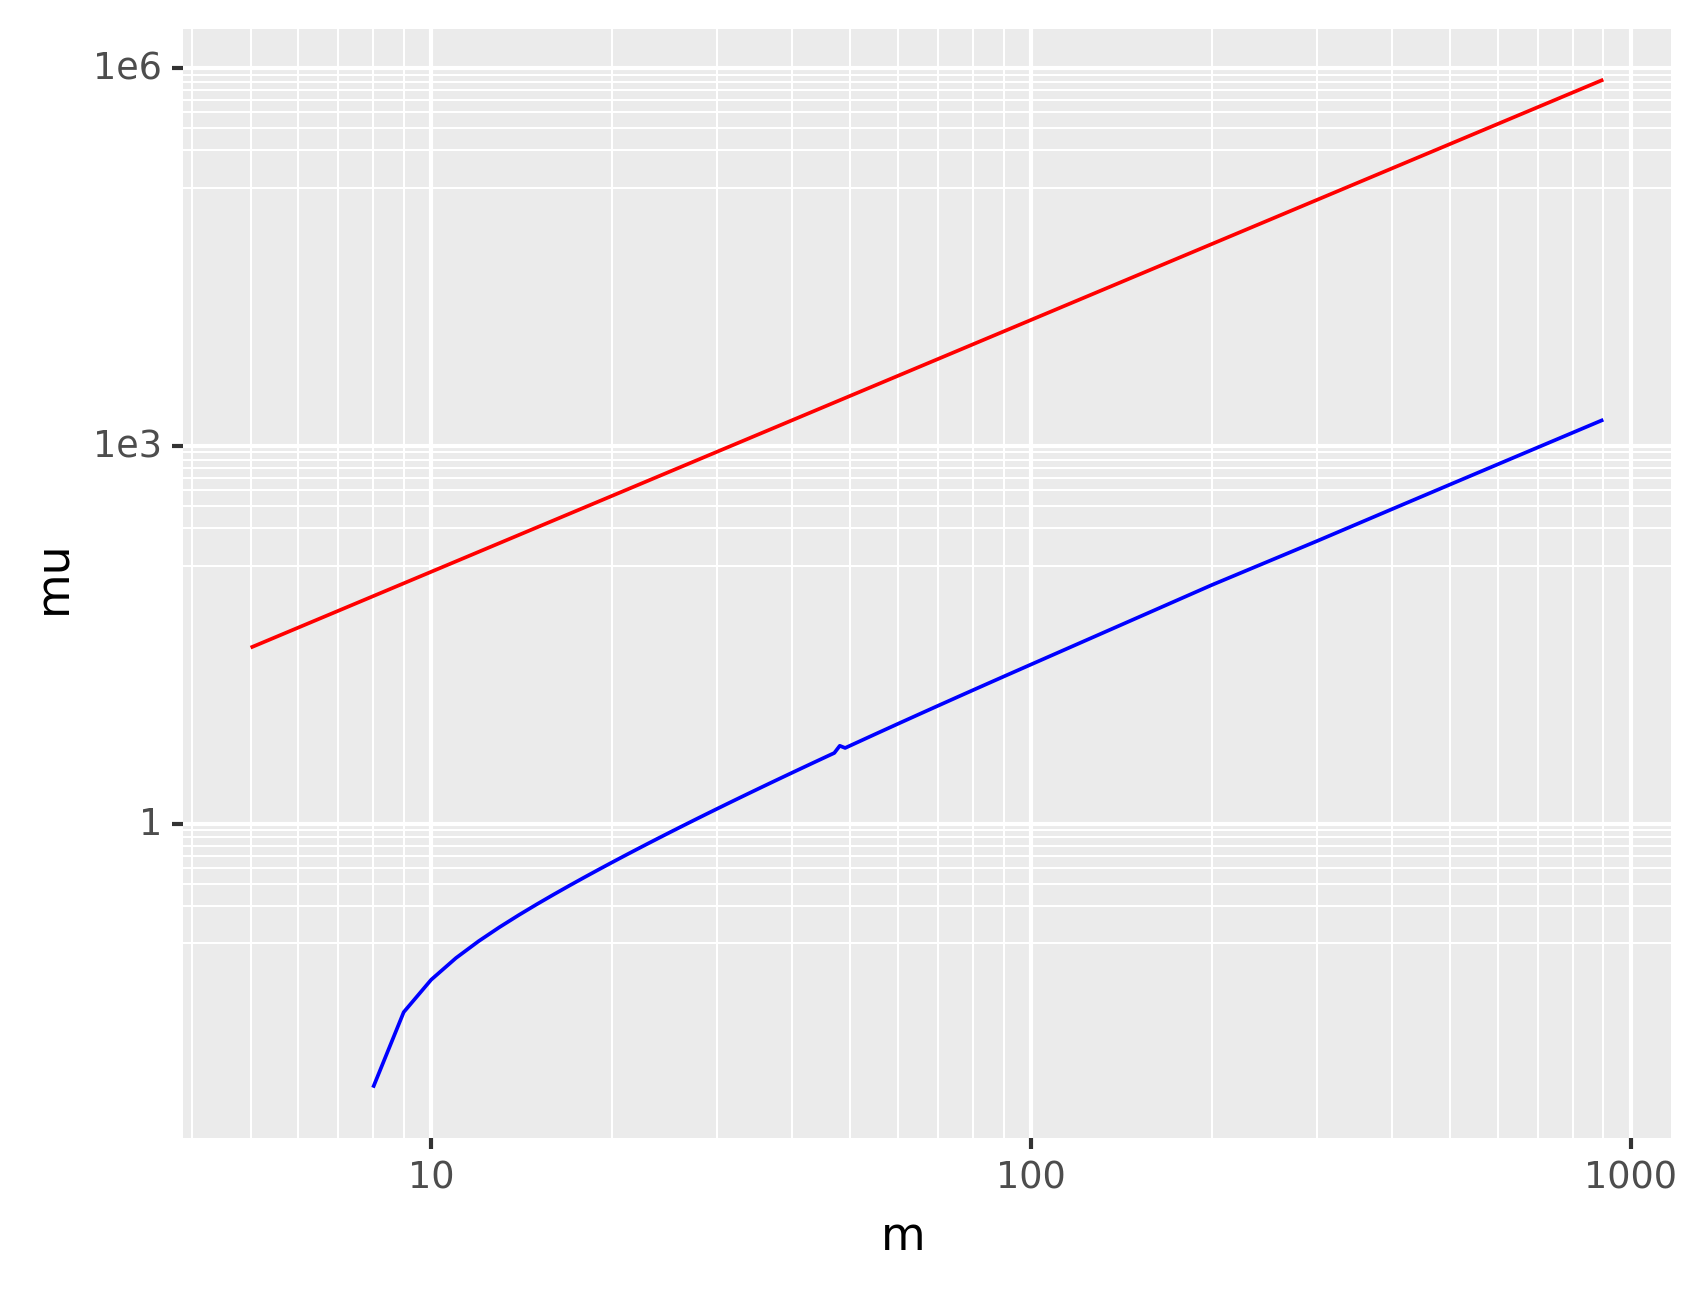
\includegraphics[width=\linewidth]{oefening3.png}
\caption{ $(\mu_{2}(A), m^2)$ vs $m$}\label{fig:muA}
\end{figure}

\oefening{4}
In dit geval is de impliciete trapezium regel:
\[
  U(t_{n+1}) = U(t_{n}) + \frac{1}{2} \tau (A U(t_{n}) + g(t_{n}) + A U(t_{n+1}) + g(t_{n+1}))
.\]
Verzamel $U(t_{n+1})$ (omdat die onbekend is) dit ziet er zo uit:
\[
  (I-\frac{\tau}{2}A)U(t_{n+1}) = U(t_{n}) + \frac{\tau}{2} (AU(t_{n}) + g(t_{n})+ g(t_{n+1}))
.\]
Dit is een ijl stelsel die een unieke oplossing heeft voor kleine $\tau$.
LU is hier de meest voor de hand liggende methode omdat we dit stelsel
herhaaldelijk moeten oplossen.

\oefening{5}
Kijk python code. (mijn script werkt niet voor $m = 200$ ik weet niet waarom
waarschijnlijk rare numerieke python dingens \ldots)

\oefening{6}
We hebben de formules geïmplementeerd maar numeriek convergeert niet naar exact.
(we hebben waarschijnlijk ergens een fout gemaakt).
\end{document}

